\subsection{21 августа. Т/б <<Глобус>>}
\textbf{Примечание:} в конце отчёта есть описание этого дня от одного из участников похода, Ильи Шалфеева.

\textit{Метеоусловия: утром, днём, вечером ясно, тепло}

\begin{figure}[h!]
	\centering
	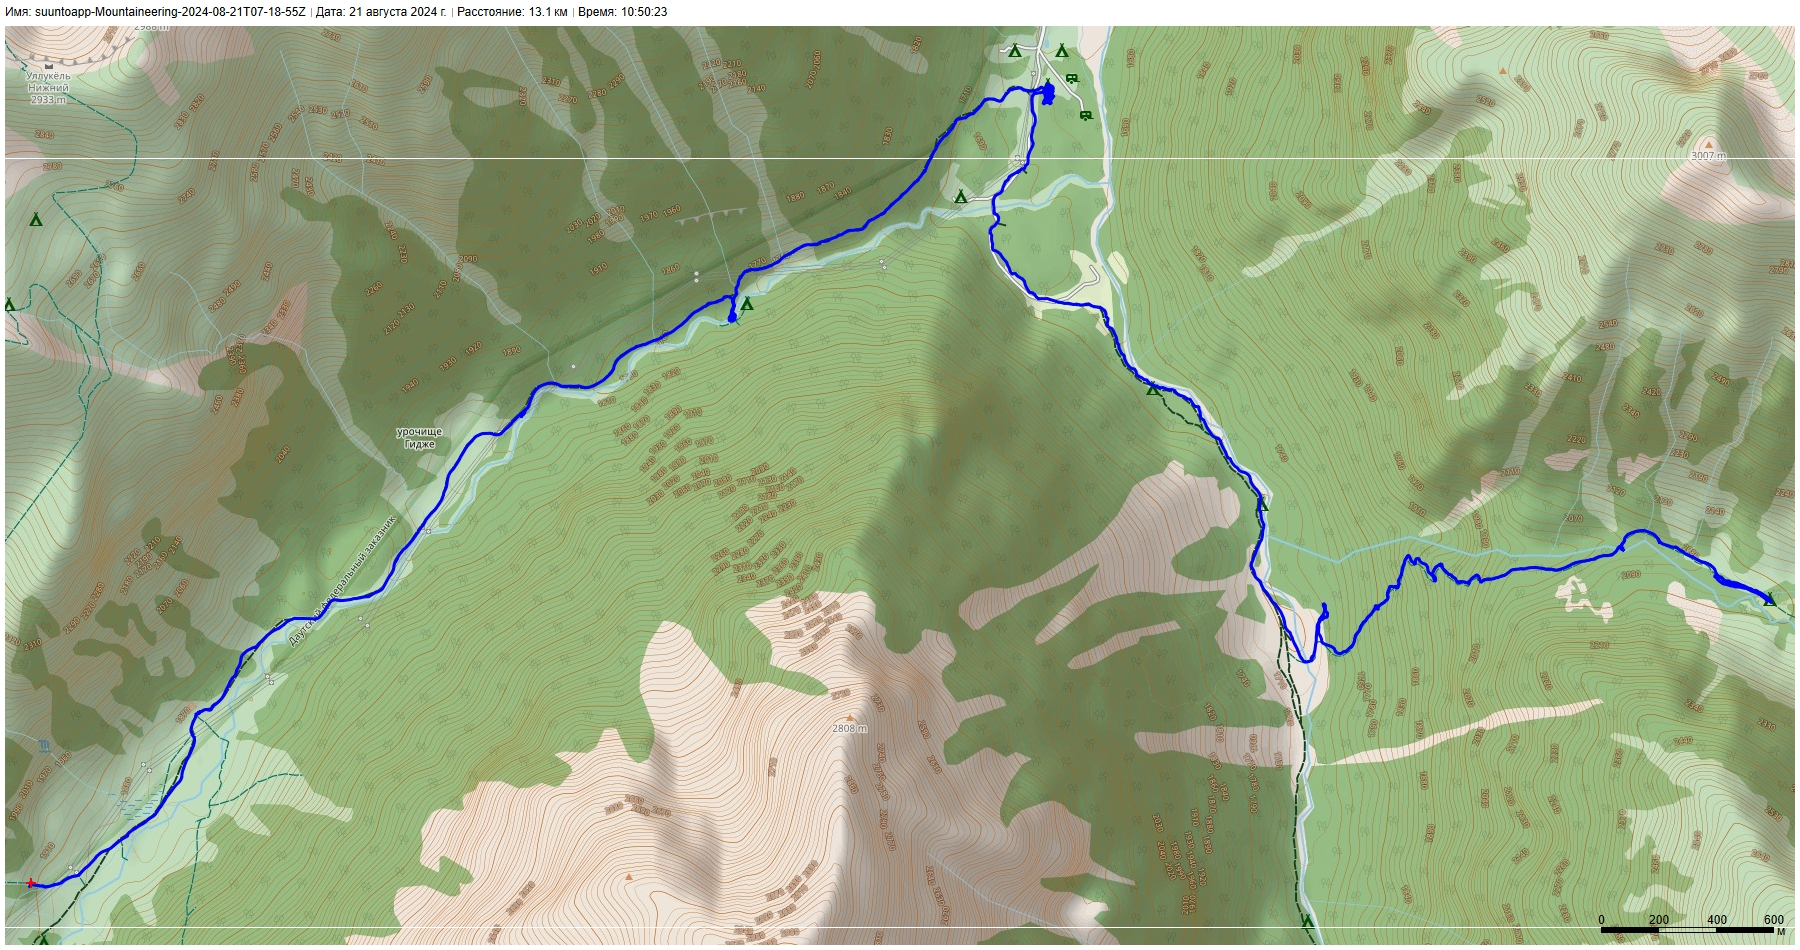
\includegraphics[angle=0, width=0.7\linewidth]{../pics/mini_maps/21}
	\label{fig:mini_21}
\end{figure}

Подъём дежурных между 07:00 и 08:00; общий подъём в 08:30. (рис.~\ref{fig:DSC_0993}). 

\begin{figure}[h]
	\centering
	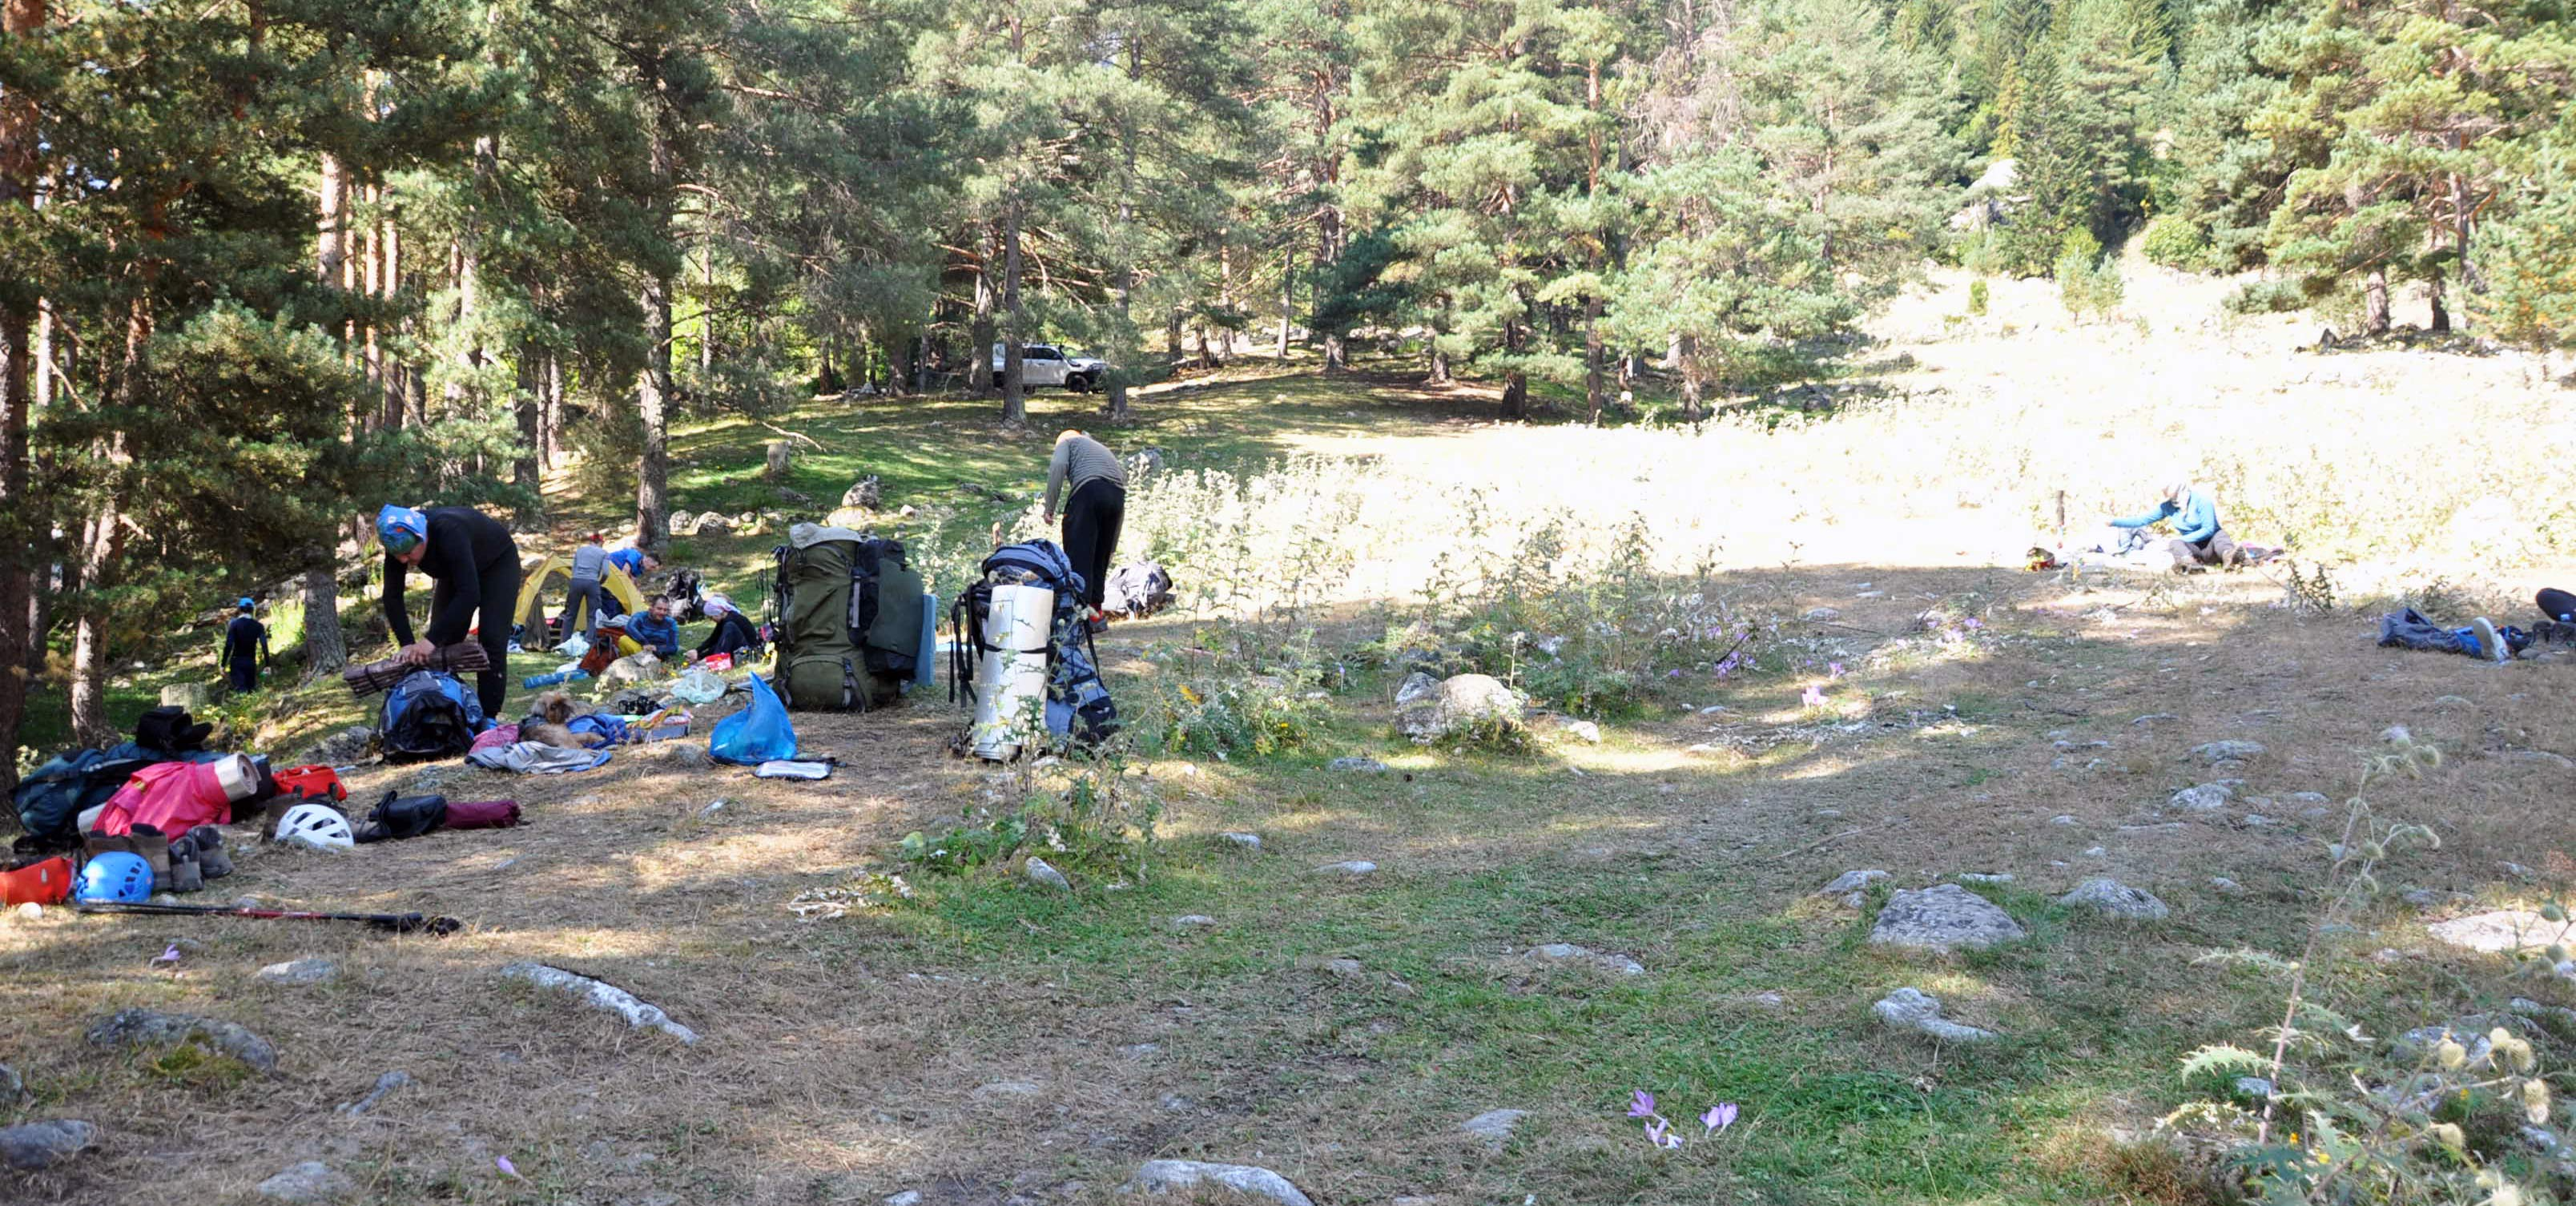
\includegraphics[width=0.7\linewidth]{../pics/DSC_0993}
	\caption{м.н. 20-21 августа}
	\label{fig:DSC_0993}
\end{figure}

Не спеша позавтракали, отдыхая от позднего завершения вчерашнего дня, и в 10:20 выдвинулись по д.р. Махар в сторону т/б <<Глобус>>(рис.~\ref{fig:DSC_1003}). 

\begin{figure}[h]
	\centering
	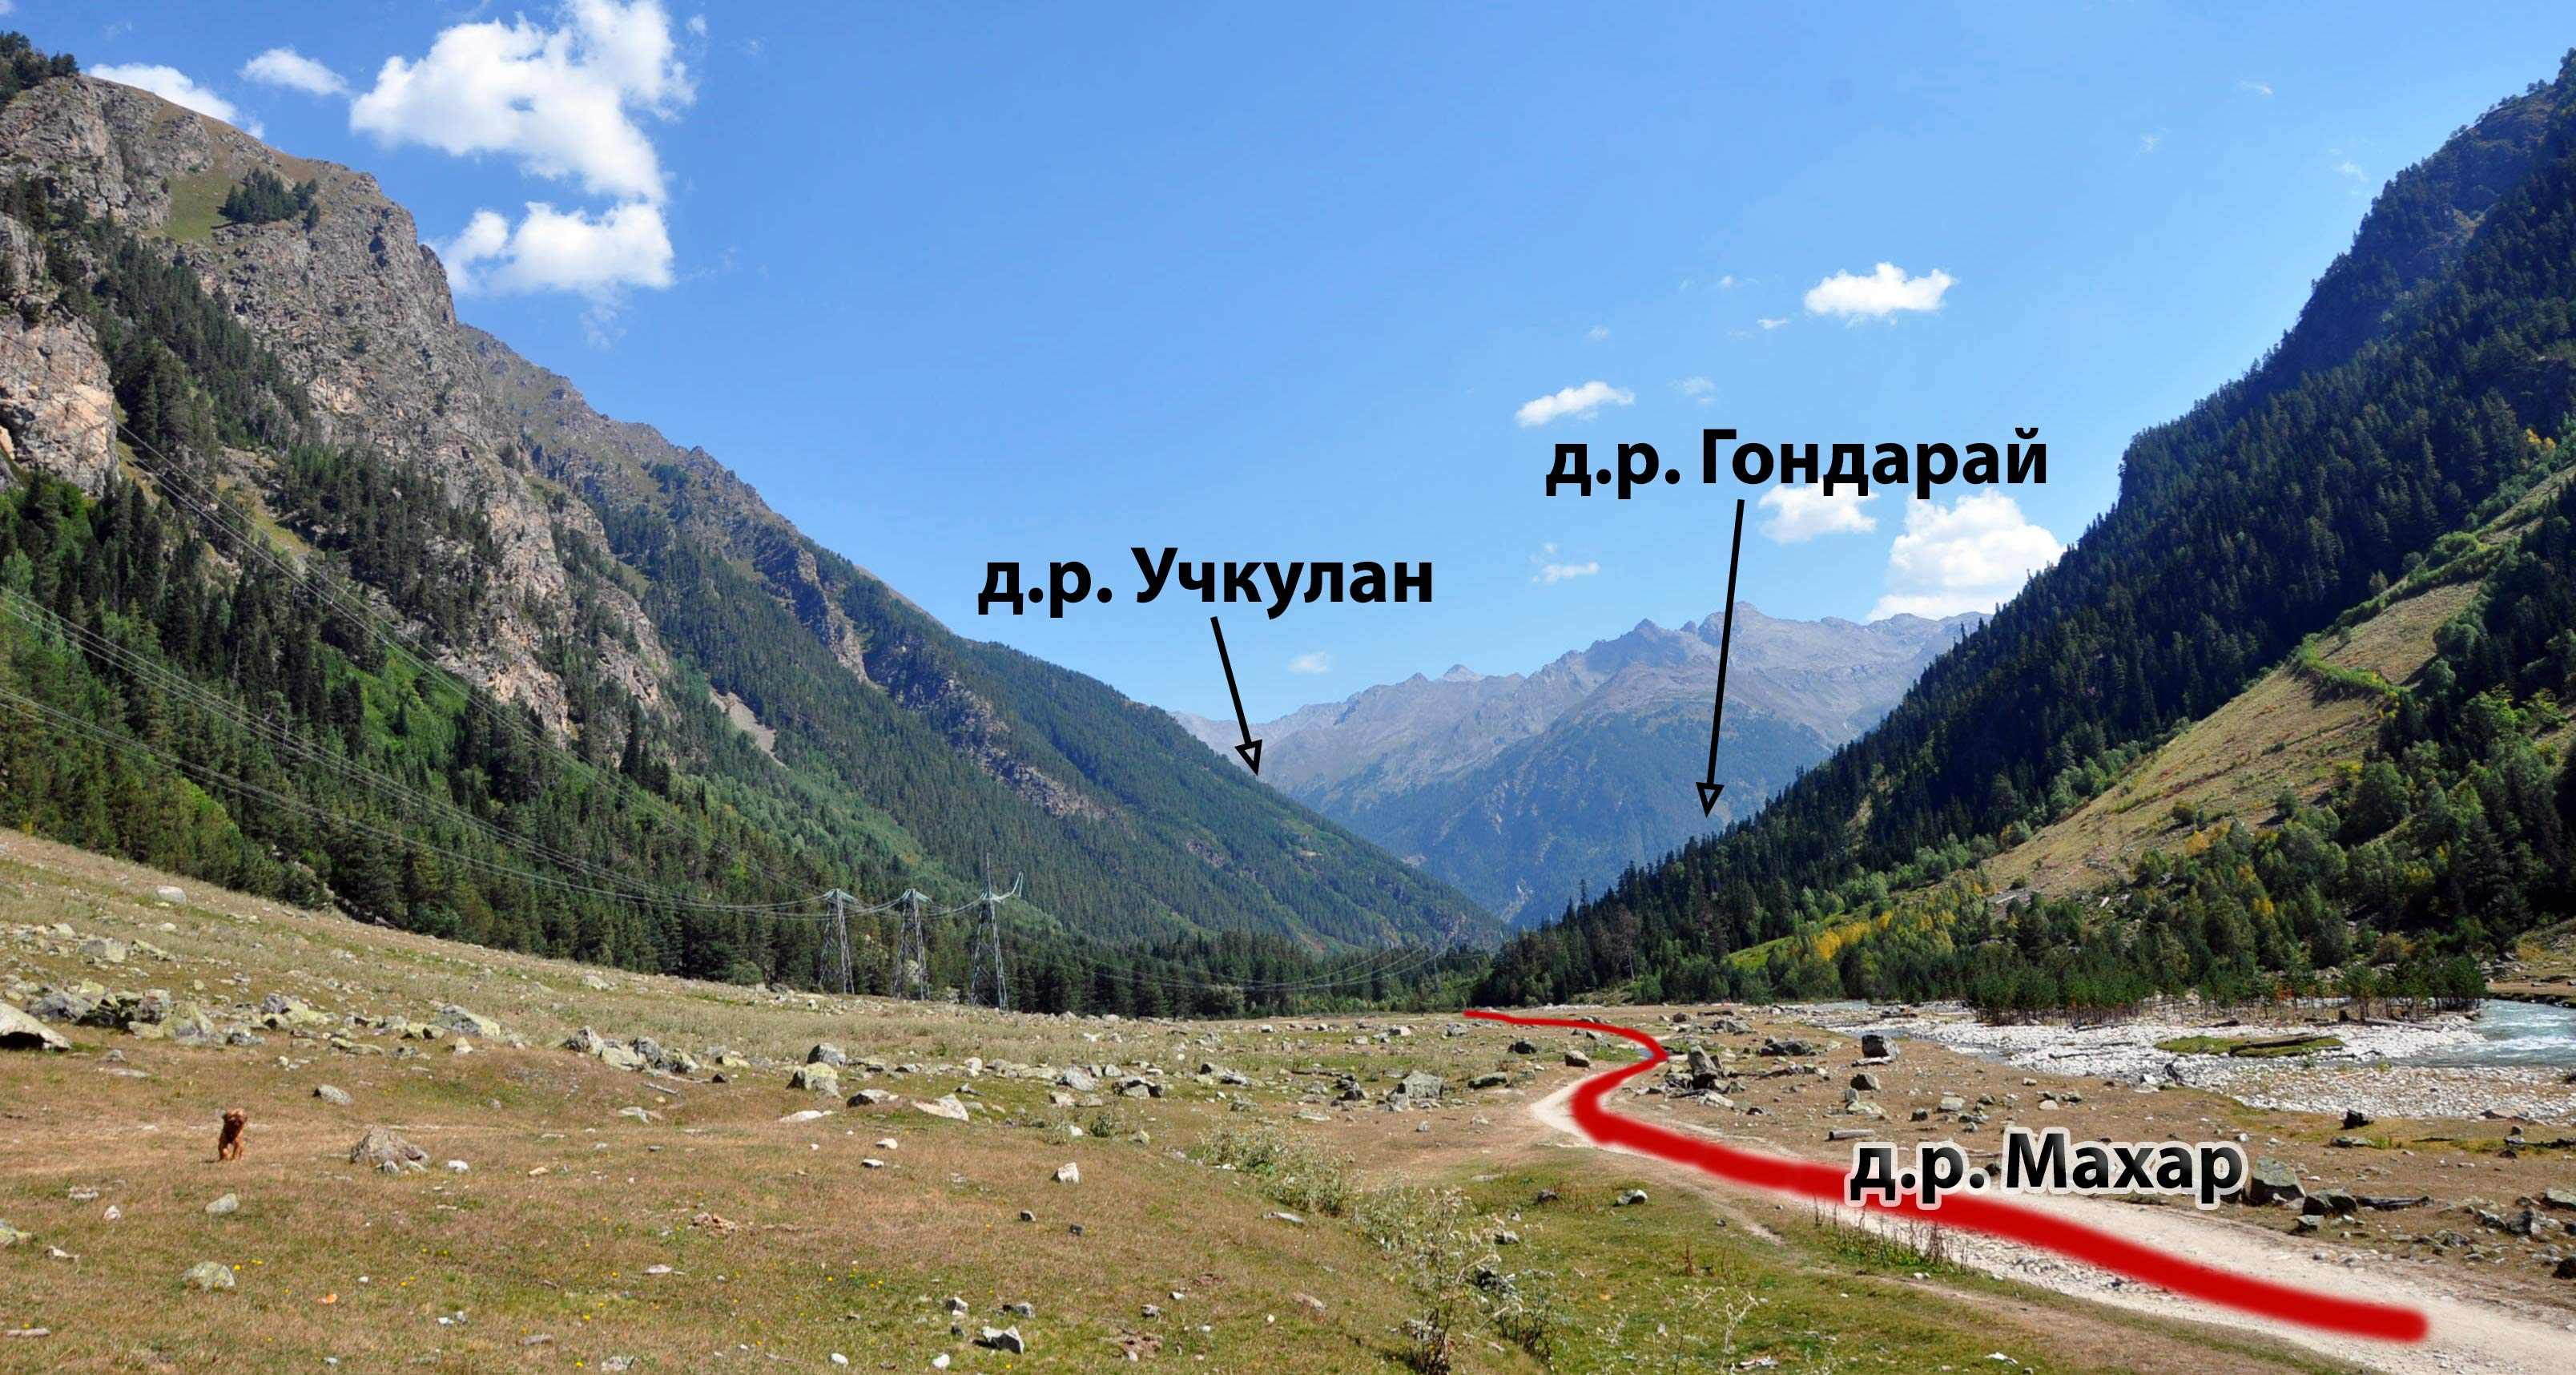
\includegraphics[width=0.7\linewidth]{../pics/DSC_1003}
	\caption{м.н. 20-21 августа}
	\label{fig:DSC_1003}
\end{figure}

Через 20~мин ЧХВ подошли к посту пограничников. Пограничники задали нам вопросы о направлении движения, сфотографировали нитку маршрута в маршрутной книжке, но документы не проверили. Выйдя от них, ещё через 22~мин ЧХВ дошли до нарзанных источников (находятся на правом берегу р. Махар, туда ведёт хороший подвесной мост, рис.~\ref{fig:DSC_1043}). Координаты источников: N43.312198\degree, E43.312198\degree.

\begin{figure}[h!]
	\centering
	\begin{minipage}[h]{0.62\linewidth}
		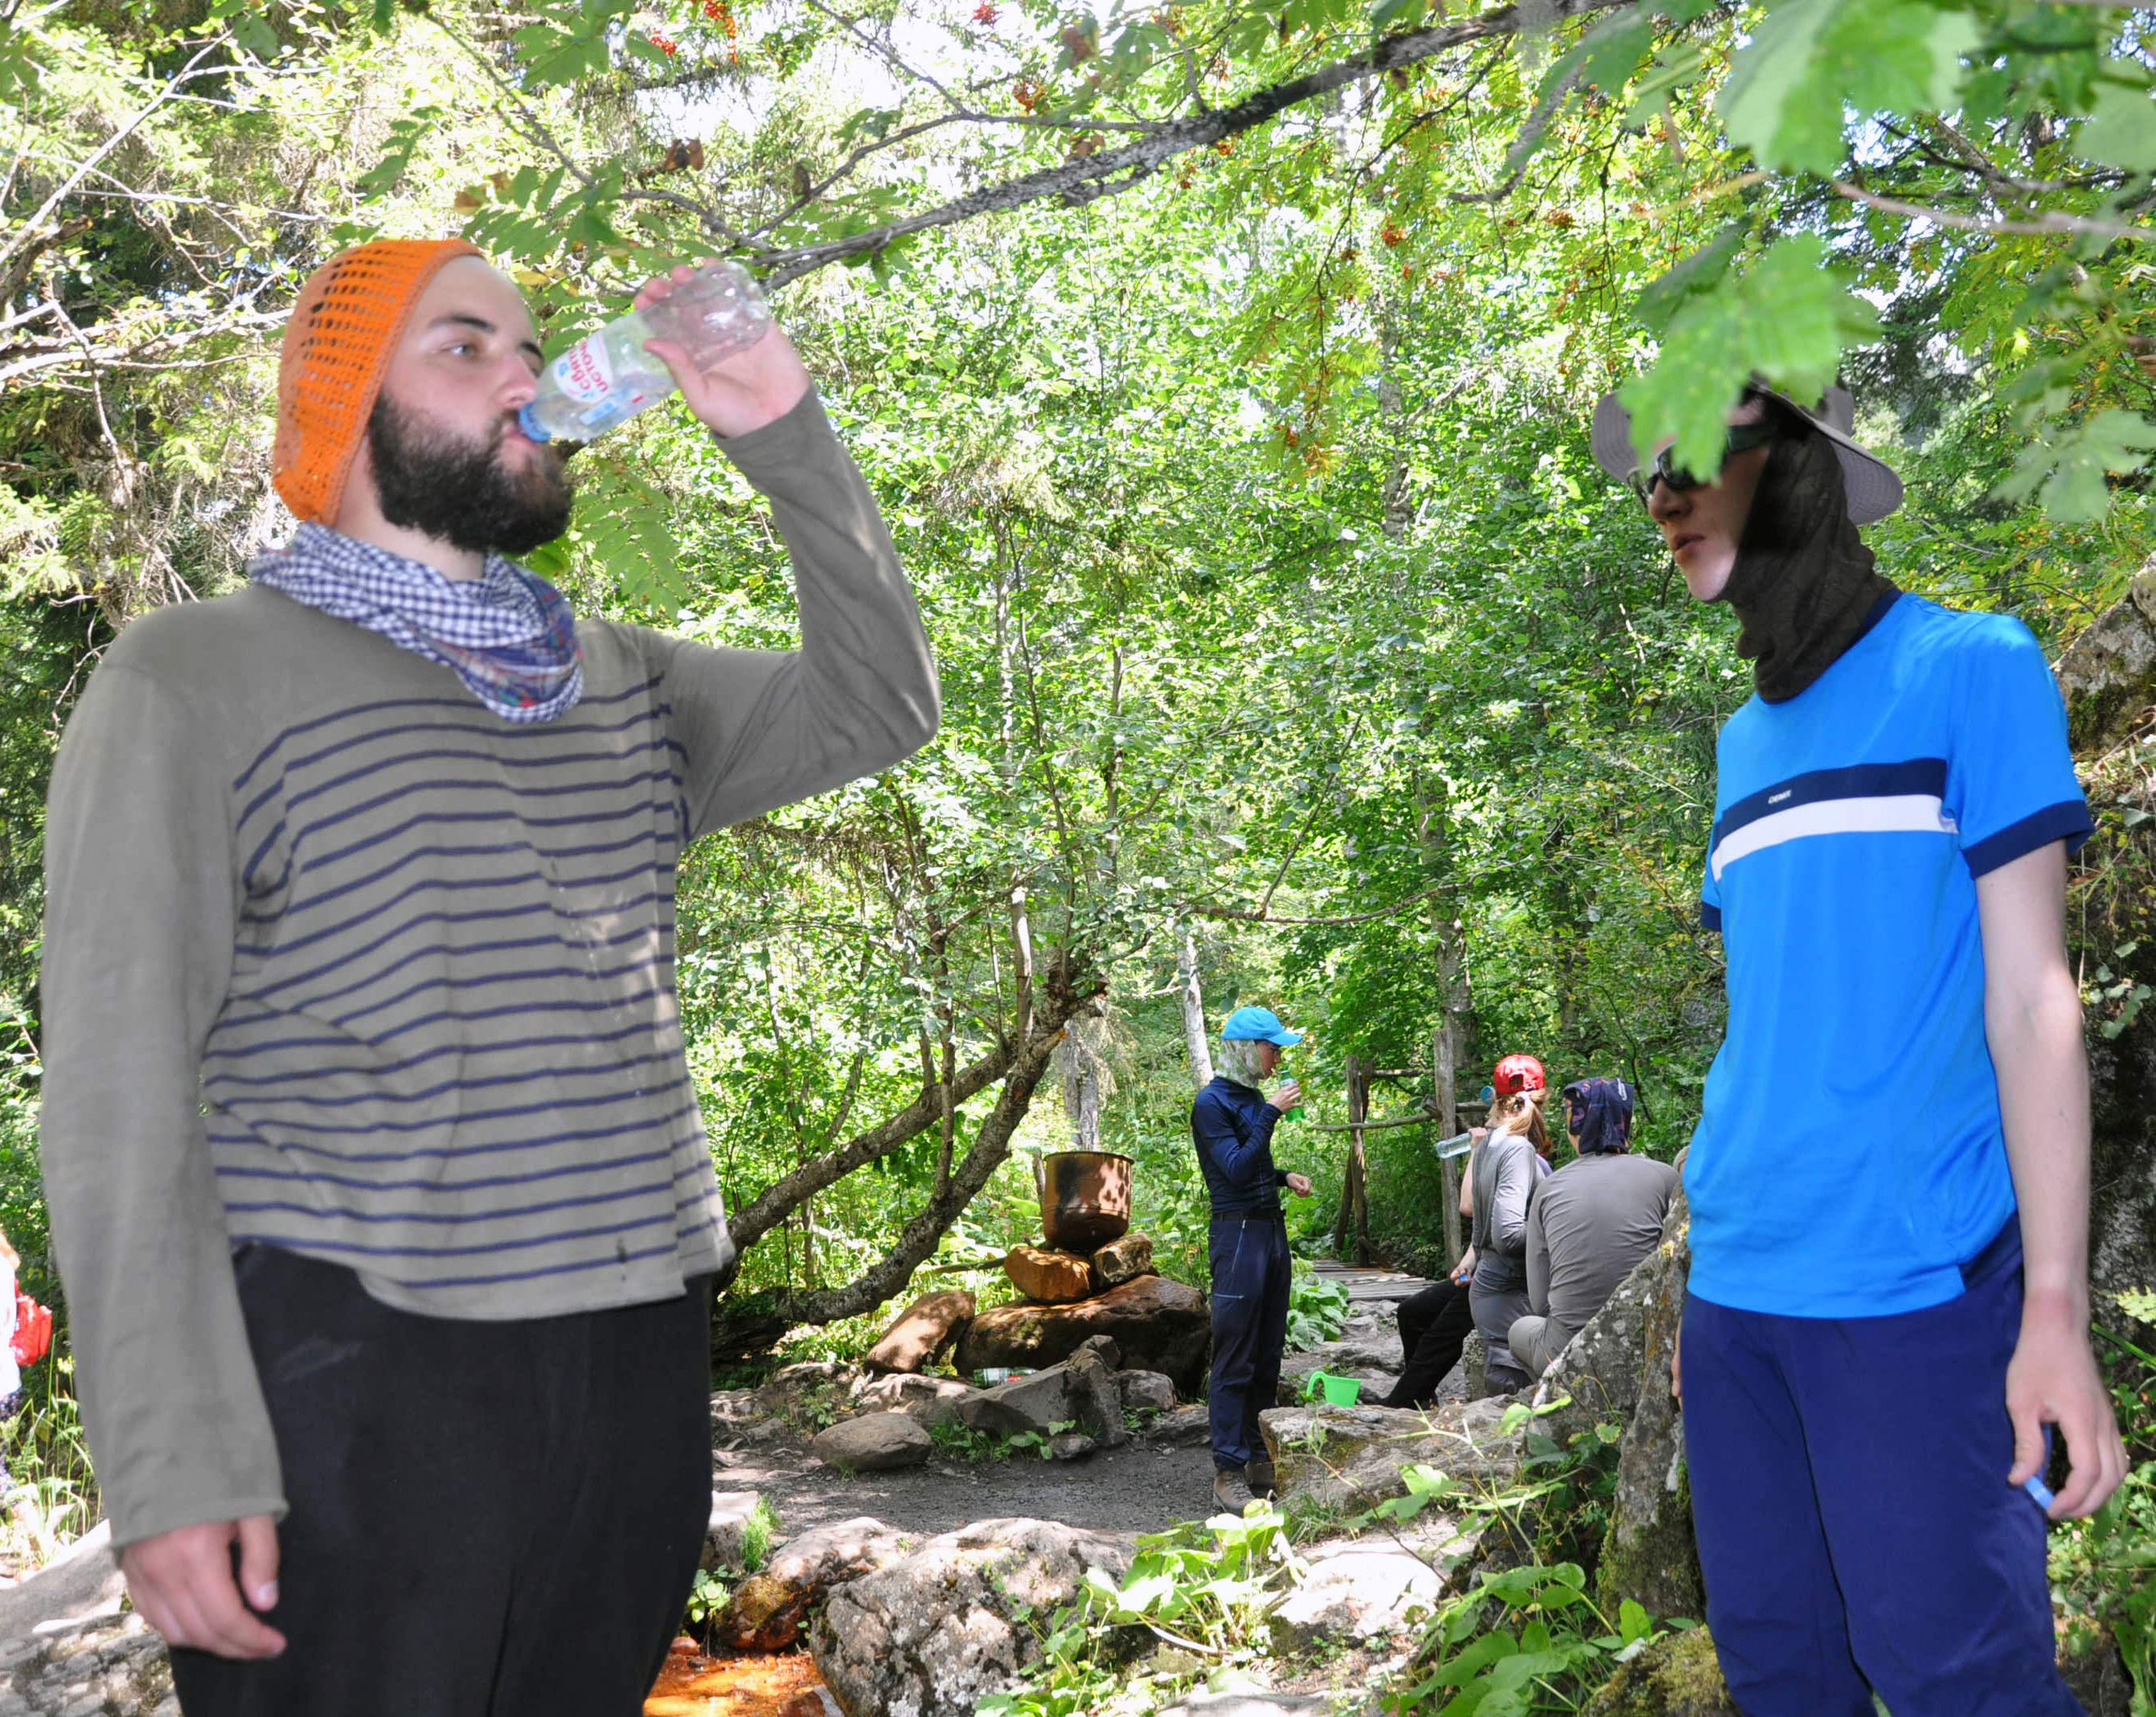
\includegraphics[width=\linewidth]{../pics/DSC_1043.jpg}
	\end{minipage}
	\quad
	\begin{minipage}[h]{0.35\linewidth}
		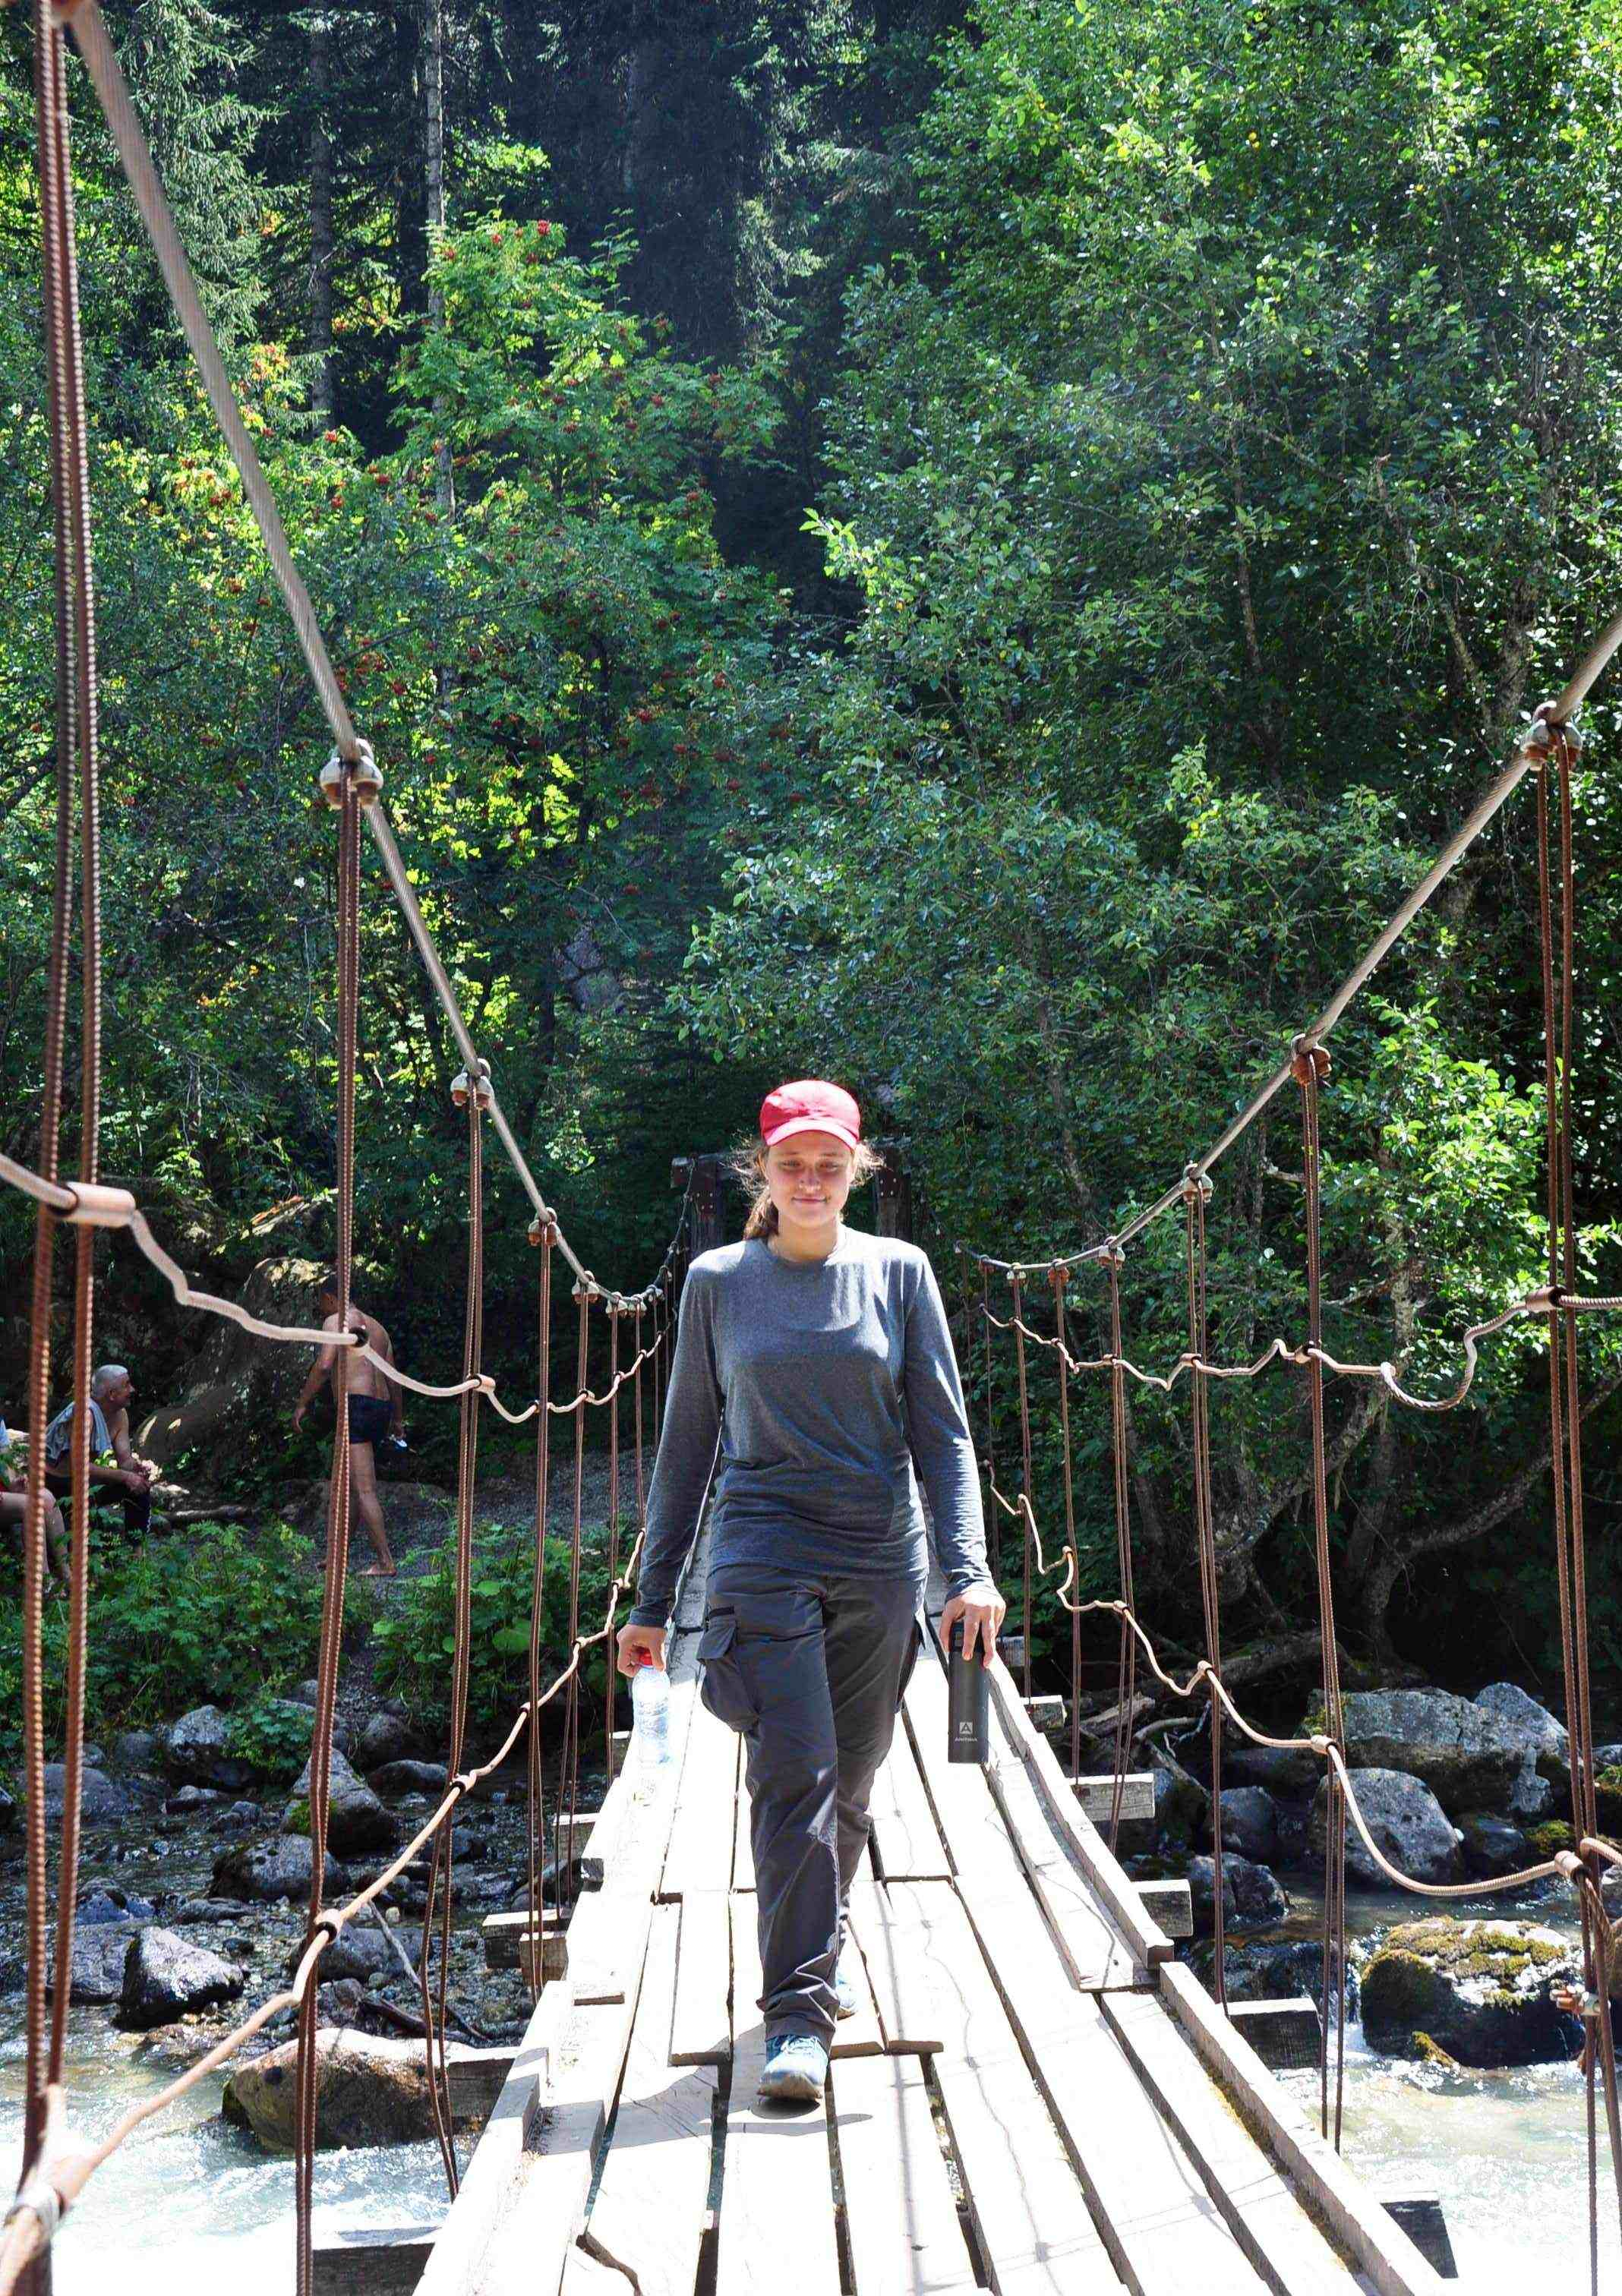
\includegraphics[width=\linewidth]{../pics/DSC_1098.jpg}
	\end{minipage}
	\caption{Слева: группа на нарзанных источниках. Справа: мост через р. Махар к источникам}
	\label{fig:DSC_1043}
\end{figure}

В 12:05 пришли в т/б <<Глобус>>, где встали на обед. Информация о благах цивилизации в турбазе: можно бесплатно подзарядить телефоны (около 5 шт одновременно, предположительно, что от солнечной батареи), при необходимости можно попросить Wi-Fi, с которого, если повезёт, получится обменяться парой сообщений с большой землёй. Также есть владелец одного из соседних кемпингов (по его собственным словам: есть подозрение, что это было не так), который за 300~\faRub~разрешил нам позвонить со своего телефона со стабильным интернетом. На территории турбазы есть душ, туалет, домики для ночлега и магазин с хычинами.

\begin{figure}[h!]
	\centering
	\begin{minipage}[h]{0.30\linewidth}
		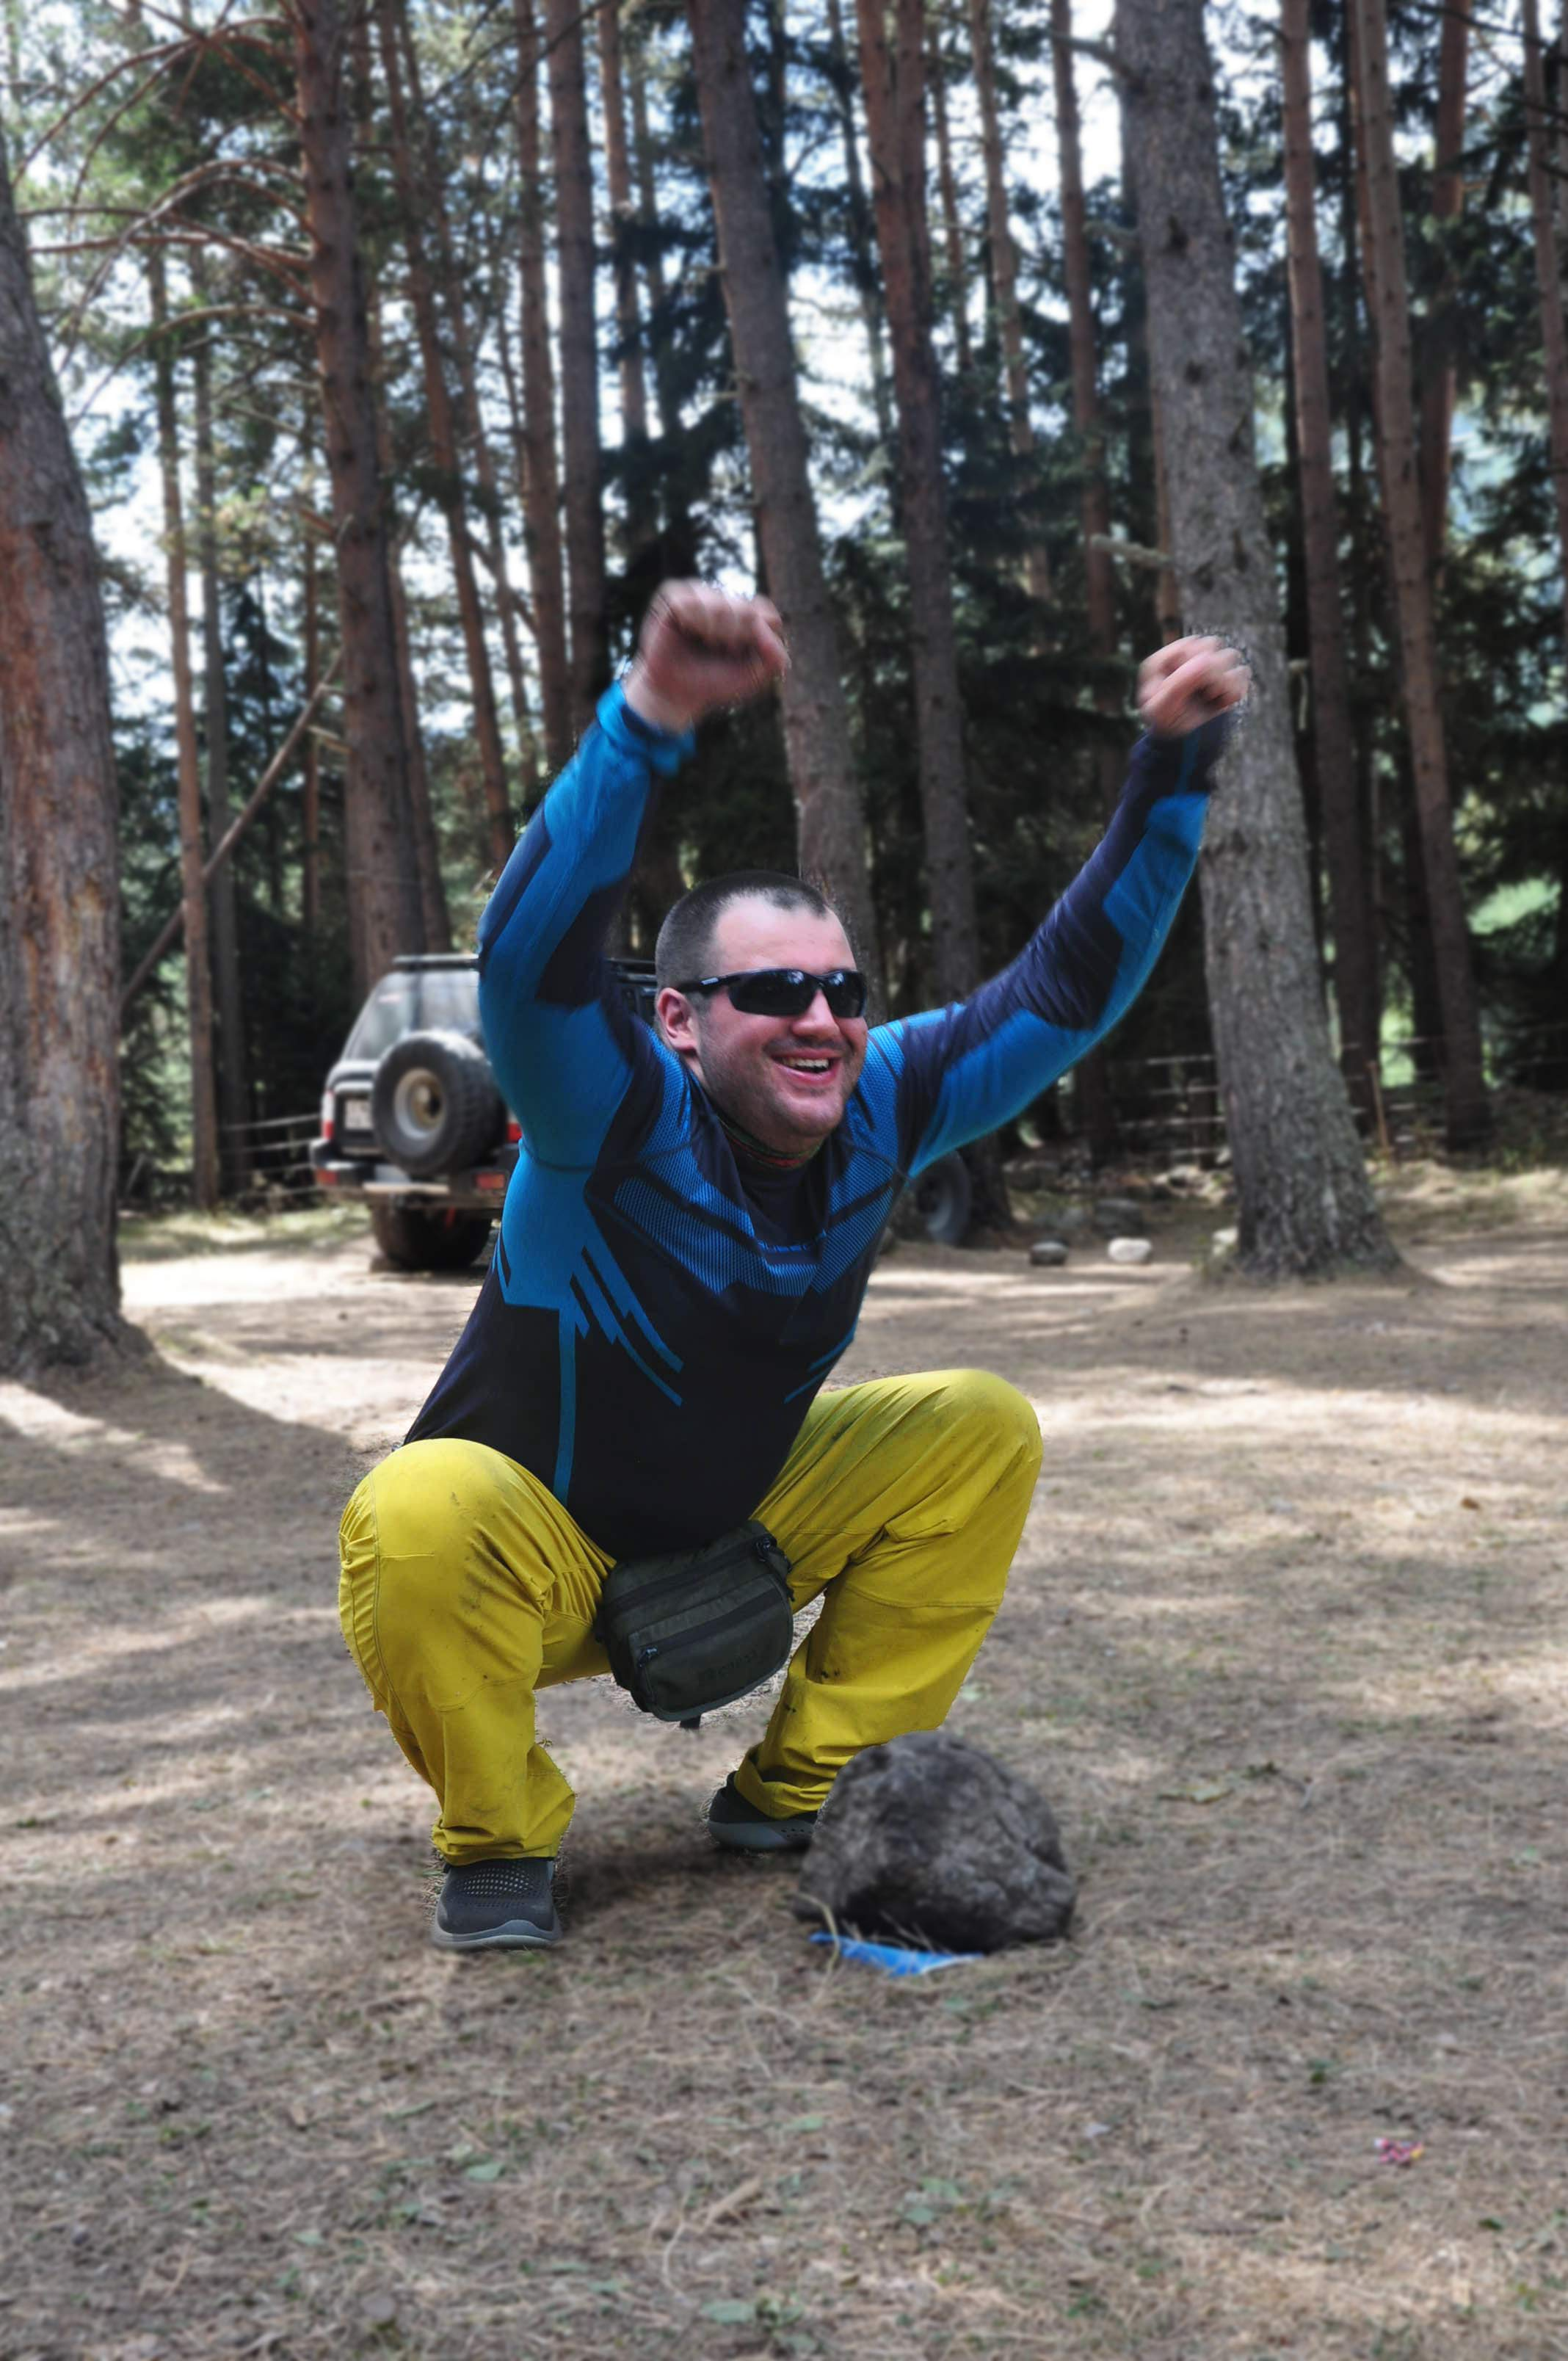
\includegraphics[width=\linewidth]{../pics/DSC_1150.jpg}
	\end{minipage}
	\quad
	\begin{minipage}[h]{0.30\linewidth}
		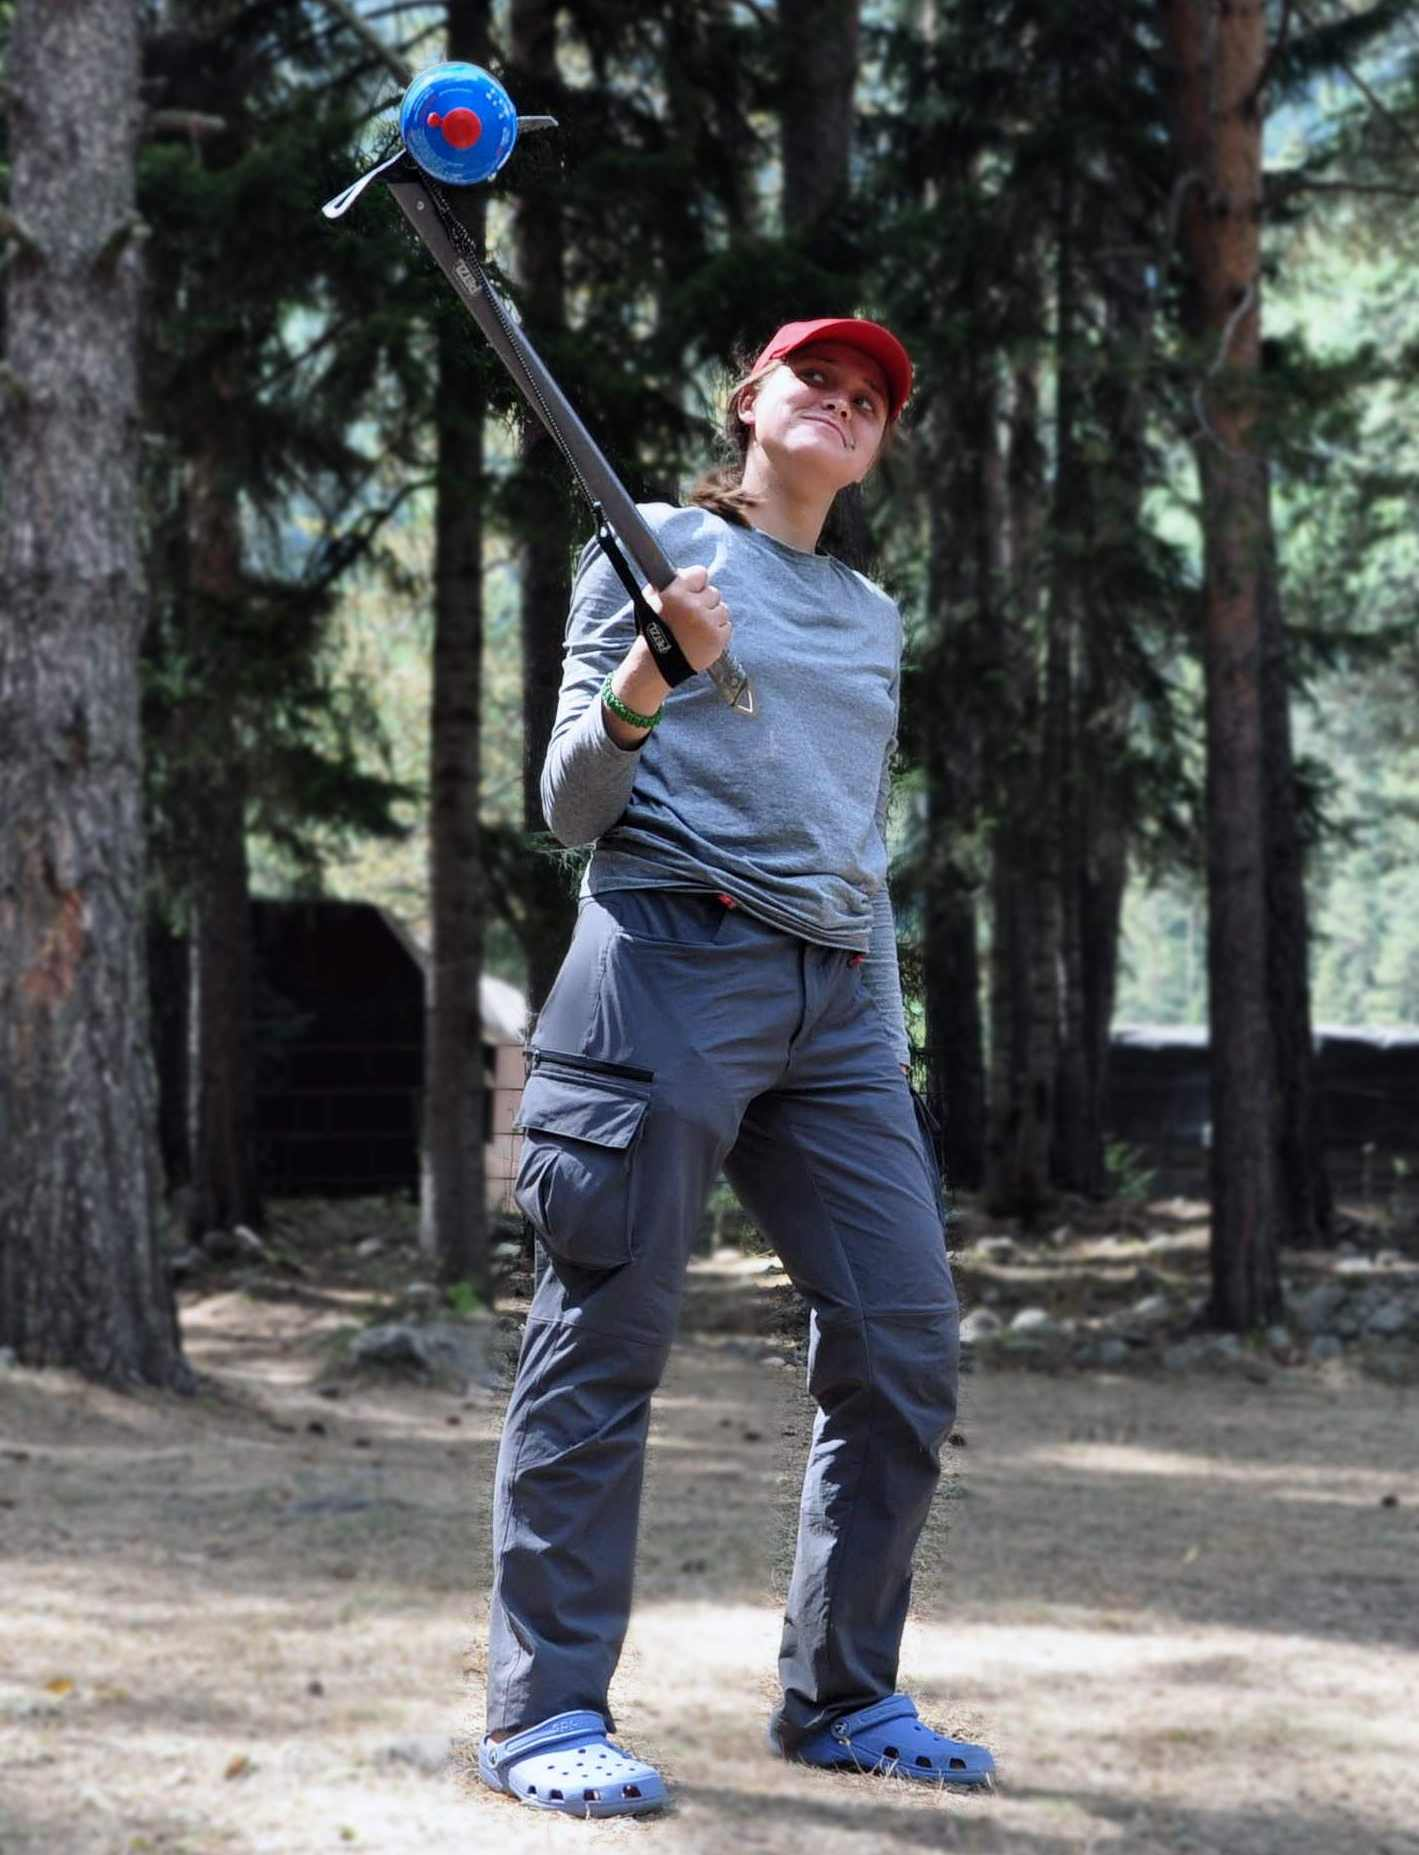
\includegraphics[width=\linewidth]{../pics/DSC_1152.jpg}
	\end{minipage}
	\caption{Учимся утилизировать использованные газовые баллоны \smiley}
	\label{fig:DSC_1150}
\end{figure}

После обеда один из участников, Георгий, сообщил группе о своём решении сойти с маршрута по причине того, что поход давался ему слишком тяжело: выявились проблемы с коленями, давлением, да и общий уровень физической подготовки, несмотря на то, что участник тренировался перед походом, оказался всё же недостаточным. На переходе до турбазы он обратился с этим к руководителю лично, и вовремя обеда вопрос обсуждался в личном порядке. Основной вклад в решение технических вопросов вносил при этом замруководителя. Времени на обеспечение логистики Георгия на большую землю ушло довольно много , и в 17:53 мы выдвинулись из турбазы по хорошей автомобильной дороге по правому берегу р. Учкулан. В 18:06 пересекли р. Махар по хорошему автомобильному мосту., а в 18:32~--- р. Гондарай по трём хорошим брёвнам (рис.~\ref{fig:hondaray}).

\begin{figure}[h]
	\centering
	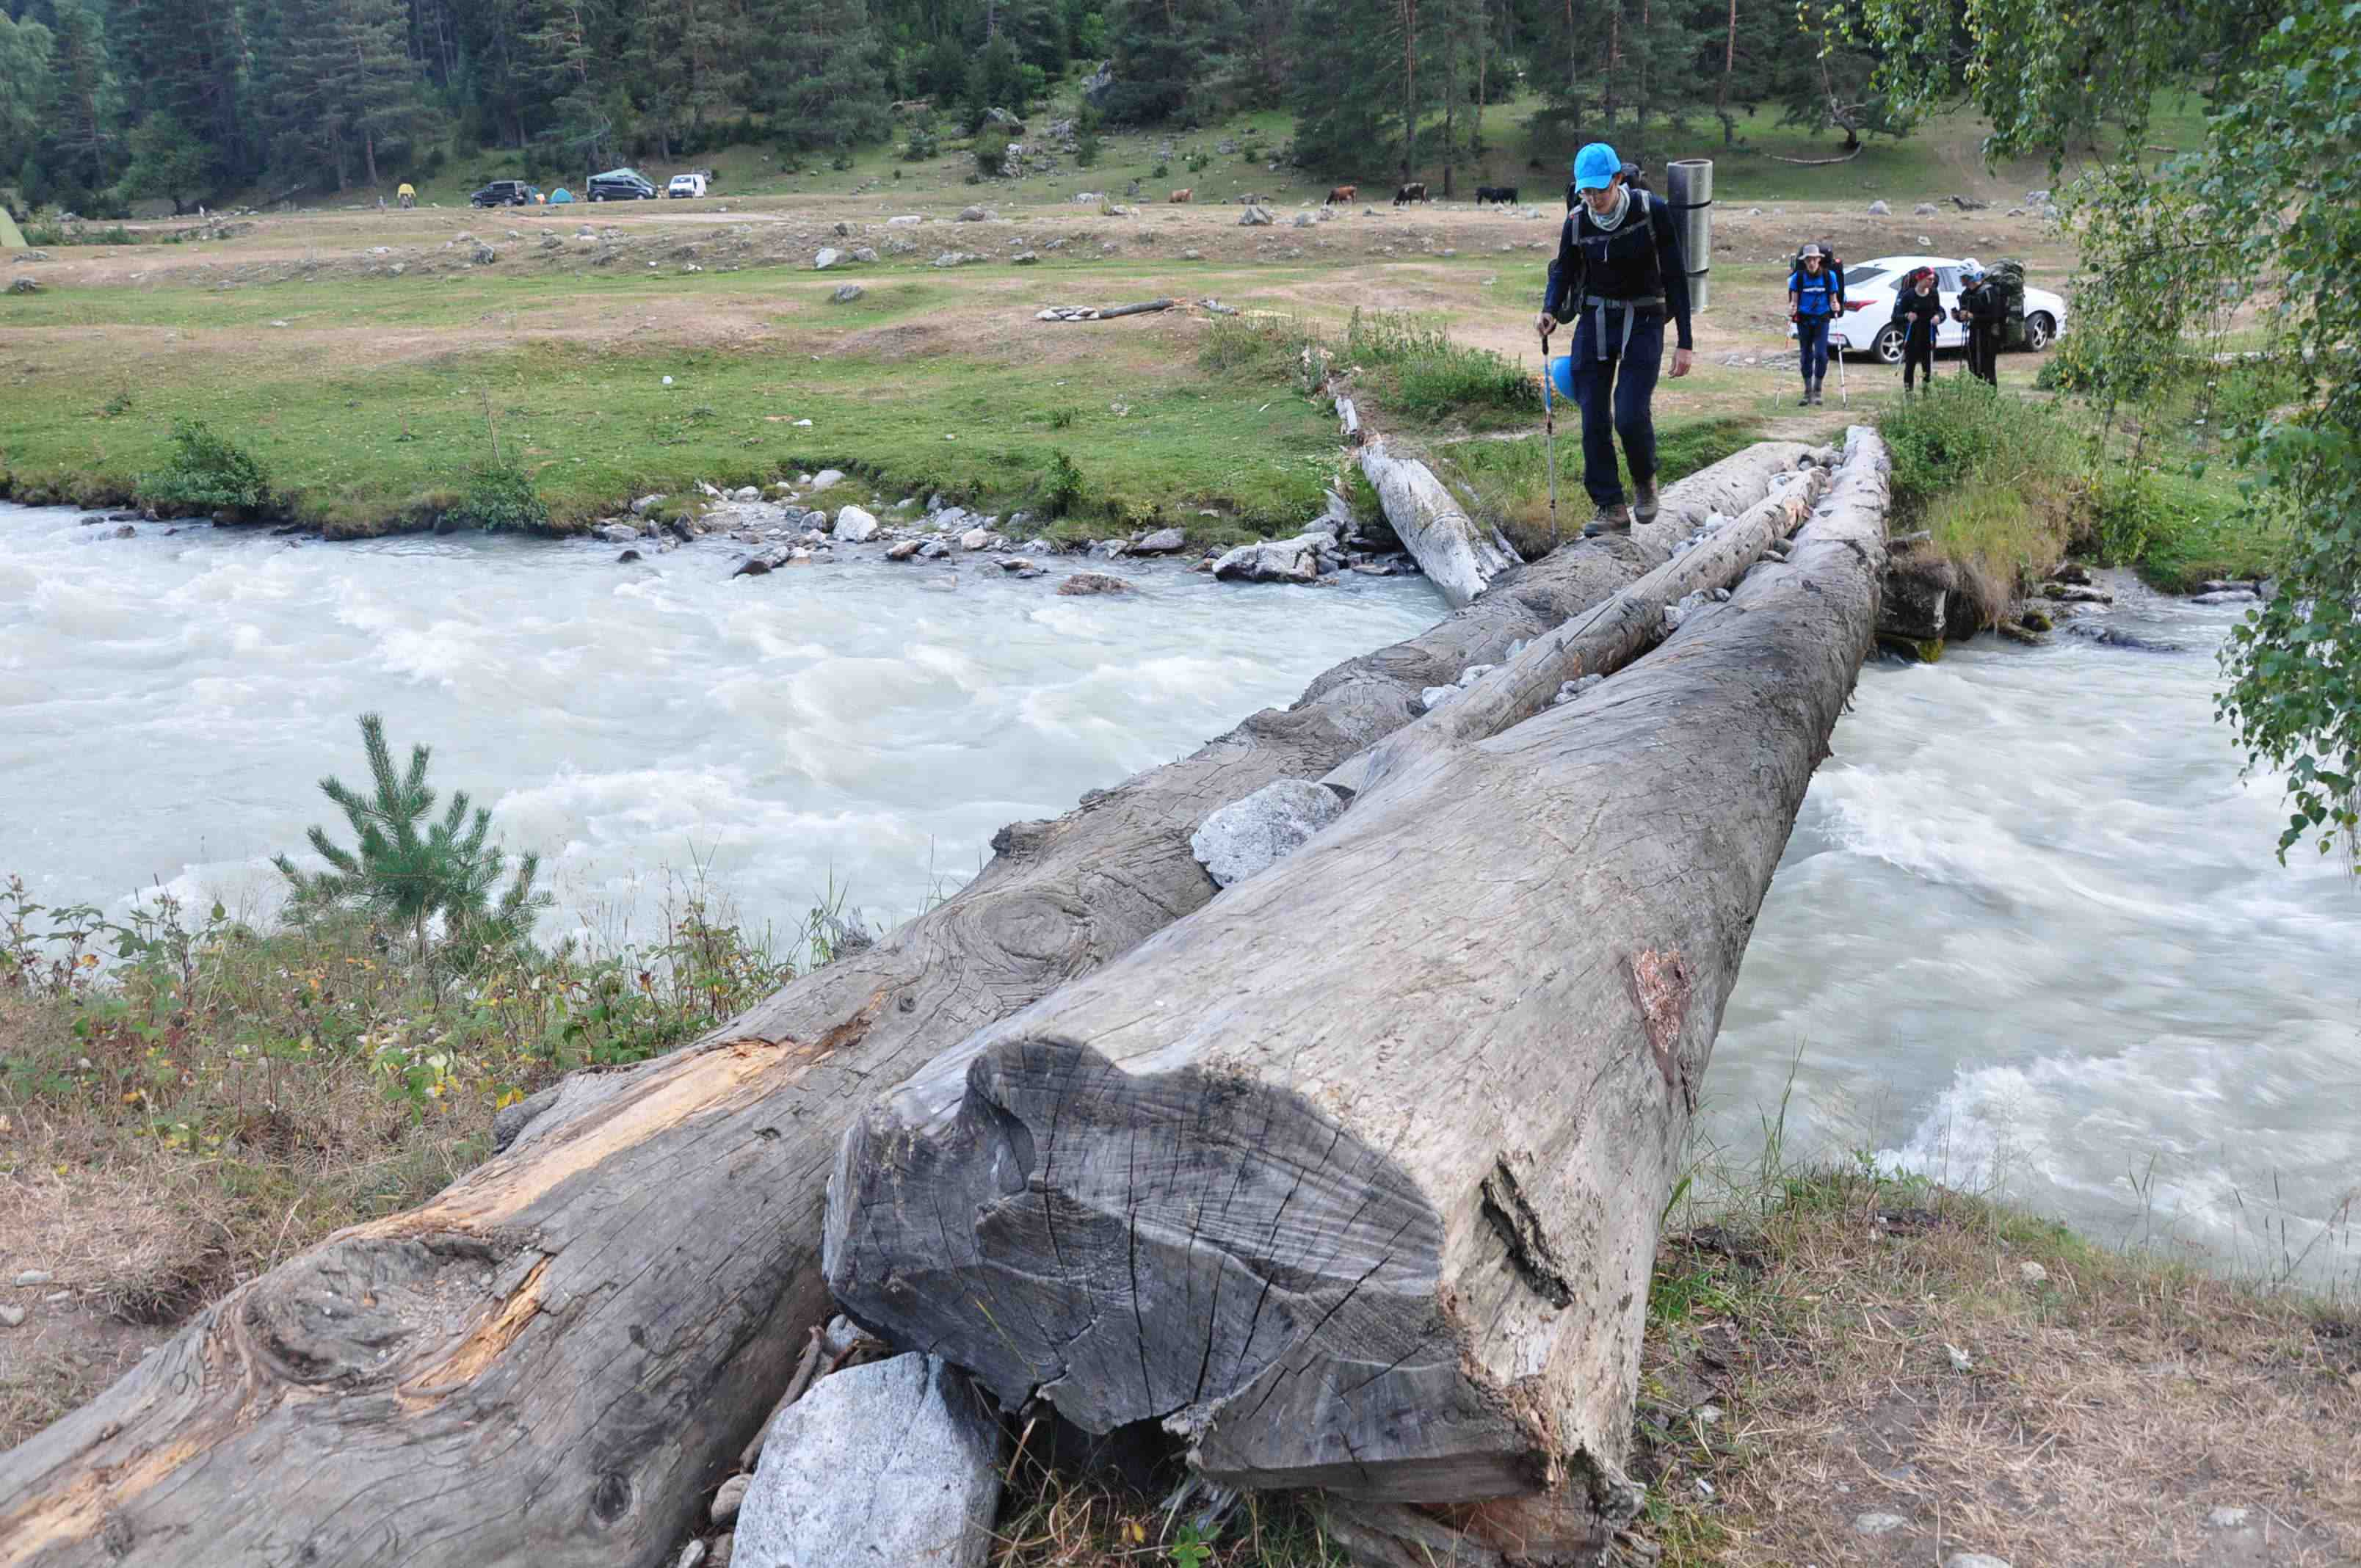
\includegraphics[width=0.7\linewidth]{../pics/DSC_1167}
	\caption{Группа пересекает р. Гондарай по мосту из бревён}
	\label{fig:hondaray}
\end{figure}

На левом берегу реки есть места для ночёвок, но мы приняли решение подняться в по лесной дороге в д.р. Джалпаккол, поскольку руководитель утверждал, что в 2018 году \cite{Korolyov2018} их группа, так же начав подниматься, в итоге развернулась, а на следующий день оказалось, что до конца подъёма не дошли совсем немного. Воспоминание оказалось ошибочным, и мы не рекомендуем последующим группам так делать. Подъём по достаточно крутой лесной дороге, переходящей в тропу, занял около двух с половиной часов, из которых 2 часа ЧХВ было в тёмное время суток с фонариками.

В 20:20 пересекли р. Джалпаккол по мосту, в 21:05 пришли на оборудованные ночёвки у правого притока Джалпаккола. Координаты м.н. N43.303453\degree,~E42.031513\degree. Стоит отметить, что за 200 м до этого места также имеются места для ночёвок, с водой, но менее сухие и удобные (координаты N43.304245\degree, E42.029190\degree).



\clearpage